\section{Candidate code list exploration} 
\label{s:codelistanalyzer}

We describe here a proof-of-concept experiment, which involves query-based exploration of candidate code lists in the LOV knowledge base, in which we can find the description of RDFS vocabularies and OWL ontologies defined for and used by datasets on the Linked Data Cloud.

The goal of this part of our research has been to create and apply a collection of SPARQL queries that can be used in the process of exploring code lists in LOV. % and other knowledge bases as well. %Another specific goal was to identify the coverage of knowledge instances with respect to their abstract concepts. 

\subsection{Query sequence for candidate code list exploration}
The detection and extraction of code lists in a vocabulary consists of several steps and five main queries. The exact parameterized SPARQL queries labeled Q1 through Q5 can also be found in the mentioned GitHub repository homepage.

For reproducibility purposes, the steps of this experiment are summarized as follows:

\begin{enumerate}
    \item Create a list of vocabularies that might contain code lists, sorted by the number of included individuals and classes.

    \item In each vocabulary, find all classes and count the number of their instances and subclasses.

    \item For each class with at least one instance, find all its instances (individuals) and check if these instances are connected to \emph{skos:Concept}, which is known to be used for code lists.

    \item Query for direct relationships between these instances and use these information to visualize the candidate code list (e.g. Figure \ref{fig:code-list-visualized})

    \item Query for the instance-instance relationships that exist in each vocabulary, including the total number of instances on both sides of the relationships (this helps to check if we missed any codes).

\end{enumerate}

Using this procedure, we collected all candidate code lists for manual review, and if a result proves to be a code list but does not use \emph{skos:Concept}, we enhance it by connecting the collected codes with \emph{skos:Concept}, and their class with \emph{skos:ConceptScheme} (using SPARQL, Code listing \ref{lst:sparql6} in the paper). The enhanced data are then compiled to one knowledge base, which provides simpler access to the code lists, because we enhanced them with SKOS.



Note that none of the queries is to be understood as a strict definition of what should be a code list.
Instead, the queries assemble collections of results that can be independently inspected and gradually produce a code list knowledge base potentially useful for the community (without guarantee that every single element would fully satisfy a rigorous or common-sense concept of what should a code list be).
The queries, especially, Q3 and Q4, are derived from the analysis presented in the previous section. 

\medskip
\medskip
\noindent\textbf{Q1: Identify the named graph IRI of the target vocabularies}. This step is done by retrieving a list of vocabulary IRIs and their names. In addition, we also query for the number of classes and instances in each vocabulary. Note that in this query we only retrieve english labels, or labels that have no specified language, of the vocabularies. The total number of vocabularies having at least one class instance in LOV was 281. Examples of results for this query are shown in Table \ref{tab:q1-results}, which lists the top vocabularies with the highest number of class instances. Note that some vocabularies are not listed here even though they include class instances. This is because this query assumes the classes have the property \textit{rdfs:isDefinedBy} so that their number can be counted for each vocabulary. This can be fixed by applying query Q0 included in our GitHub repository README before running query Q1, but this requires setting up a custom endpoint with enabled SPARQL UPDATE. The number of classes and instances indicates the probability of code lists existing in each vocabulary and helps to set the priority for analyzing each vocabulary. Vocabularies that have a low number of classes and instances will less probably include code lists. %This way, the analysis procedure would find the majority of code lists in the targeted knowledge base sooner.

\begin{lstlisting}[captionpos=b, caption=Q1 -- Query to get a list of ontologies with number of classes and number of class instances,label=lst:sparql1,basicstyle=\ttfamily,frame=single]
SELECT DISTINCT ?u ?p ?l 
       (COUNT(DISTINCT ?c) AS ?nc) 
       (COUNT(DISTINCT ?i) AS ?ni) {
  ?u a voaf:Vocabulary .
  ?u vann:preferredNamespacePrefix ?p .
  VALUES ?labelProp { 
     rdfs:label dc:title
     dcterms:title skos:prefLabel
  }
  OPTIONAL {
    ?u ?labelProp ?l .
    FILTER(
      LANGMATCHES(LANG(?l), 'en') || 
      LANGMATCHES(LANG(?l), '')
    )
  }
  VALUES ?class { rdfs:Class owl:Class }
  ?c a ?class . ?c rdfs:isDefinedBy ?u .
  OPTIONAL {
    ?i a ?c . ?i rdfs:isDefinedBy ?u .
  }
} GROUP BY ?u ?p ?l ORDER BY DESC(?ni)
\end{lstlisting}

\begin{table}[h]
\footnotesize
\centering
\begin{tabular}{|l|l|r|r|}
\hline
\textbf{Prefix} & \textbf{Name}                                                                 & \textbf{Classes} & \textbf{Inst.} \\ \hline
mil             & The Muninn Military Ontology                                                  & 140              & 618            \\ \hline
lexinfo         & LexInfo                                                                       & 183              & 271            \\ \hline
odrl            & ODRL Version 2.2                                                              & 27               & 130            \\ \hline
sh              & SHACL Vocabulary                                                              & 40               & 79             \\ \hline
voag            & Vocabulary Of Attribution                                                     & 65               & 76             \\ \hline
akt             & AKT Reference Ontology                                                        & 152              & 62             \\ \hline
mv              & MobiVoc: Open Mobility Vocab                                                  & 23               & 61             \\ \hline
spv             & Scholarly Papers Vocabulary                                                   & 9                & 50             \\ \hline
gr              & The GoodRelations Vocabulary                                                  & 32               & 46             \\ \hline
chord           & The Chord Ontology                                                            & 8                & 43             \\ \hline
txn             & TaxonConcept Ontology                                                         & 81               & 36             \\ \hline
qudt            & Quantities, Units, Dimensions                                                 & 83               & 32             \\ \hline
music           & Music Vocabulary                                                              & 108              & 30             \\ \hline
fel             & A Fine-grained Entity Linking                                                 & 28               & 24             \\ \hline
ofrd            & Fridge and Freezer Vocabulary                                                 & 8                & 24             \\ \hline
dataid          & DataID                                                                        & 17               & 23             \\ \hline
a-loc           & Location Ontology                                                             & 22               & 20             \\ \hline
vaem            & Vocabulary for Attaching                                                      & 8                & 18             \\ \hline
hydra           & The Hydra Core Vocabulary                                                     & 1                & 17             \\ \hline
gleif-L2        & Global Legal Entity                                                           & 9                & 17             \\ \hline
vvo             & VVO: The Volkswagen Vehicles                                                  & 16               & 16             \\ \hline
%oa              & Web Annotation Ontology                                                       & 21               & 15             \\ \hline
%opo             & OnlinePresence Ontology                                                       & 14               & 14             \\ \hline
% mo              & The Music Ontology                                                            & 54               & 13             \\ \hline
%akts            & AKT Reference Ontology                                                        & 17               & 13             \\ \hline
% vso             & VSO: The Vehicle Sales                                                        & 28               & 12             \\ \hline
% gleif-L1        & Global Legal Entity Identifier                                                & 12               & 11             \\ \hline
% lib             & Experimental  with Schema.org                                                 & 16               & 10             \\ \hline
% cwork           & Creative Work Ontology                                                        & 6                & 10             \\ \hline
% bbc             & BBC Ontology                                                                  & 5                & 10             \\ \hline
\end{tabular}
\caption{Q1 result excerpt (modified)} \label{tab:q1-results}.
%\vspace{-6mm}
\end{table}

\medskip
\noindent\textbf{Q2: Get a list of instantiated classes with the number of their instances}. From a vocabulary (whose IRI is the parameter of this query), we retrieve classes that have at least one instance. The number of instances tells us the size of the expected candidate code list. We assume that the code list members could be referenced by other entities; we thus also query for the incoming property edge and its domain entity. This means that the class is on the side of the range of the edge. During the collection, we observed that not many code lists have predefined assignment properties and we presume that these instances are probably not meant to be code lists. They could be just ad hoc instances added to the ontology for the illustration of the classes, or because they are considered important in the domain. These cases should be further analyzed based on the meanings of these instances. Result examples for query Q2 are shown in Table \ref{tab:q2-results}.

\begin{lstlisting}[captionpos=b, caption=Q2 -- Query to get the number of instances of each class in an ontology with their range properties and domain classes,label=lst:sparql2,basicstyle=\ttfamily,frame=single]
SELECT ?d ?p ?c (COUNT(DISTINCT ?i) AS ?ni)
FROM <${ontology}> 
WHERE {
  VALUES ?t {
    rdfs:Class
    owl:Class
  }
  ?c a ?t .
  ?i a ?c .
  OPTIONAL { 
    ?p rdfs:range ?c . 
    OPTIONAL { ?p rdfs:domain ?d . }
  }
}
GROUP BY ?d ?p ?c
ORDER BY DESC(?ni)
\end{lstlisting}

\begin{table}[ht]
\footnotesize
\centering
\begin{tabular}{|l|l|l|r|}
\hline
\textbf{Domain}  & \textbf{Property} & \textbf{Code list} & \textbf{Codes} \\ \hline
mil:PostToUnit   & mil:toUnit        & mil:MilitaryRank           & 605              \\ \hline
foaf:Person      & mil:heldRank      & mil:MilitaryRank           & 605              \\ \hline
org:Organizat.   & mil:rankOf        & mil:MilitaryRank           & 605              \\ \hline
                 &                   & mil:Rank                   & 45               \\ \hline
                 &                   & mil:Soldier                & 34               \\ \hline
                 &                   & mil:MilitaryTrade          & 18               \\ \hline
                 &                   & mil:MilitaryAppo.          & 14               \\ \hline
                 &                   & mil:ArmsType               & 8                \\ \hline
                 &                   & mil:BattleSpace            & 5                \\ \hline
                 &                   & mil:Non-Combat.            & 2                \\ \hline
                 &                   & mil:Role                   & 1                \\ \hline
\end{tabular}
\caption{Q2 result excerpt for the Military Ontology (modified)} \label{tab:q2-results}
%\vspace{-6mm}
\end{table}

\medskip
\medskip
\medskip
\noindent\textbf{Q3: Get a list of candidate code list members}. This query gives us the overview of all members of candidate code lists. Here, we retrieve the instances and subclasses of each class in each vocabulary. The vocabulary and the class are the two parameters of this query. The query results are not yet considered code lists, but are understood as a mixture of class instances found inside each ontology. In this query, we also look for whether a code list member is tagged with \emph{skos:Concept}. The fact that the code list members are \emph{skos:Concept} instances makes it easier to reference them from other knowledge graphs; thanks to \emph{skos:Concept}, the code list can be effectively extracted as a standalone resource (described in Section \ref{s:skos_codelist_collecting}). Examples of results for this query are shown in Table \ref{tab:q3-results}.

\begin{lstlisting}[captionpos=b, caption=Q3 -- Query to get a list of candidate code list members and whether it's a \textit{skos:Concept},label=lst:sparql3,basicstyle=\ttfamily,frame=single]
SELECT DISTINCT ?i (BOUND(?s) AS ?sc) ?n
FROM <${ontology}> 
WHERE {
  VALUES ?labelProp { 
     rdfs:label dc:title
     dcterms:title skos:prefLabel
  }
  ?i a <${class}> .
  ?i ?labelProp ?n . 
  OPTIONAL {
    BIND(skos:Concept AS ?s) .
    ?i a ?s .
  }
}
\end{lstlisting}

\begin{table}[h]
\footnotesize
\centering
\begin{tabular}{|l|c|l|}
\hline
\textbf{Code} & \textbf{skos:Concept} & \textbf{Name} \\ \hline
mil:1AIFRankCaptain       & true                   & Captain       \\ \hline
mil:1AIFRankGunner        & true                   & Gunner        \\ \hline
mil:1AIFRankPrivate       & true                   & Private       \\ \hline
mil:1AIFRankEngineer      & true                   & Engineer      \\ \hline
mil:1AIFRankNurse         & true                   & Nurse         \\ \hline
mil:1AIFRankCorporal      & true                   & Corporal      \\ \hline
mil:1AIFRankTrooper       & true                   & Trooper       \\ \hline
mil:1AIFRankChaplain      & true                   & Chaplain      \\ \hline
mil:1AIFRankSergeant      & true                   & Sergeant      \\ \hline
mil:1AIFRankDriver        & true                   & Driver        \\ \hline
mil:1AIFRankMajor         & true                   & Major         \\ \hline
mil:1AIFRankSapper        & true                   & Sapper        \\ \hline
\end{tabular}
\caption{Q3 result excerpt for class \textit{mil:Soldier} in the Military ontology (modified)} \label{tab:q3-results}
%\vspace{-6mm}
\end{table}

\medskip
\noindent\textbf{Q4: In each candidate code list, get all code list members' data including the relationships between them}. This last step is to construct the candidate code list as a whole. For that, we need to query for all information about the code list members. As we have mentioned before, a code list can simply have a flat structure, but it can also form a shallow hierarchy via properties such as \textit{skos:broader} or \textit{owl:subClassOf}\footnote{\label{note:owlSubClass}The properties \textit{owl:subClassOf} and \textit{owl:subClass} do not exist in the OWL specification, they are however used in the Military ontology. This is probably a mistake made by the authors. We understand that these properties should be \textit{skos:broader} or \textit{rdfs:subClassOf} according to the meanings of the codes, similarly in case of \textit{org:rankEquivalentTo}, \textit{org:rankSeniorToTransitive}, \textit{org:rankJuniorToTransitive} in Table \ref{tab:q5-results} and some others}. The query results in Table 4 show an example this particular finding. Figure \ref{fig:code-list-with-hierarchy} illustrates the visualization of such a code list structure.


\begin{lstlisting}[captionpos=b, caption=Q4 -- Query to get candidate code list structure,label=lst:sparql4,basicstyle=\ttfamily,frame=single]
SELECT DISTINCT ?c ?cn ?i1 ?i1n ?p ?i2 ?i2n
FROM <${ontology}> 
WHERE {
  VALUES ?labelProp { 
     rdfs:label dc:title
     dcterms:title skos:prefLabel
  }
  BIND(<${class}> AS ?c) . ?i1 a ?c .
  OPTIONAL { 
    ?c ?labelProp ?cn . 
    FILTER(LANGMATCHES(LANG(?cn), 'en')) 
  }
  OPTIONAL { 
    ?i1 ?labelProp ?i1n . 
    FILTER(LANGMATCHES(LANG(?i1n), 'en'))
  }
  OPTIONAL {
    ?i2 a ?c . ?i1 ?p ?i2 .
    OPTIONAL { 
      ?i2 ?labelProp ?i2n . 
      FILTER(LANGMATCHES(LANG(?i2n), 'en')) 
    }
  }
} ORDER BY ?i1
\end{lstlisting}

\begin{table}[ht]
\footnotesize
\centering
\begin{tabular}{|l|l|l|}
\hline
\textbf{Code 1}             & \textbf{Relationship} & \textbf{Code 2}             \\ \hline
2nd Corporal                &                   &                             \\ \hline
2nd Lieutenant              & owl:subClassOf\cref{note:owlSubClass}    & Lieutenant                  \\ \hline
Able Seaman                 &                   &                             \\ \hline
Air Mechanic                &                   &                             \\ \hline
Air Mechanic Class I        & owl:subClassOf\cref{note:owlSubClass}    & Air Mechanic                \\ \hline
Air Mechanic Class II       & owl:subClassOf\cref{note:owlSubClass}    & Air Mechanic                \\ \hline
Lieutenant                  &                   &                             \\ \hline
Sapper                      &                   &                             \\ \hline
Sergeant                    &                   &                             \\ \hline
Sergeant Major              &                   &                             \\ \hline
Signaler                    &                   &                             \\ \hline
Staff Sergeant              &                   &                             \\ \hline
\end{tabular}
\caption{Q4 result for class \textit{mil:Soldier} (modified)} \label{tab:q4-results}
%\vspace{-6mm}
\end{table}

\medskip
\noindent\textbf{Q5: Get a distinct list of properties that connect two code list members}. Optionally, we can verify our results using an additional query that will retrieve all properties connecting the two code list members. Examples of the results for this query are shown in Table \ref{tab:q5-results} which includes the number of connected subjects and objects via a particular predicate.

\begin{lstlisting}[captionpos=b, caption=Q5 -- Query to get list of properties that connect class instances and the number of instances on both sides,label=lst:sparql5,basicstyle=\ttfamily,frame=single]
SELECT (COUNT(DISTINCT ?i1) AS ?ni1) ?p 
       (COUNT(DISTINCT ?i2) AS ?ni2)
FROM <${ontology}> 
WHERE {
  ?c1 a owl:Class .
  ?c2 a owl:Class .
  ?i1 a ?c1 .
  ?i2 a ?c2 .
  ?i1 ?p ?i2 .
}
GROUP BY ?p
\end{lstlisting}


\begin{table}[h]
\footnotesize
\centering
\begin{tabular}{|r|l|r|}
\hline
\textbf{Subj. Codes}       & \textbf{Property}                   & \textbf{Obj. Codes}       \\ \hline
416                        & owl:subClass\cref{note:owlSubClass} & 157                       \\ \hline
1                          & owl:disjointWith                    & 1                         \\ \hline
41                         & org:rankEquivalentTo*               & 41                        \\ \hline
35                         & org:rankSeniorToTransitive*         & 36                        \\ \hline
39                         & mil:rankOf                          & 5                         \\ \hline
33                         & skos:inScheme                       & 5                         \\ \hline
1                          & skos:broader                        & 1                         \\ \hline
36                         & org:rankJuniorToTransitive*         & 35                        \\ \hline
\end{tabular}
\footnotesize
\caption{Q5 results for the Military Ontology (modified)\\ \**\textit{these properties do not exist in the Core Organization ontology}} \label{tab:q5-results}
%\vspace{-6mm}
\end{table}


\begin{figure}[h]
\centering
%\captionsetup{justification=centering}
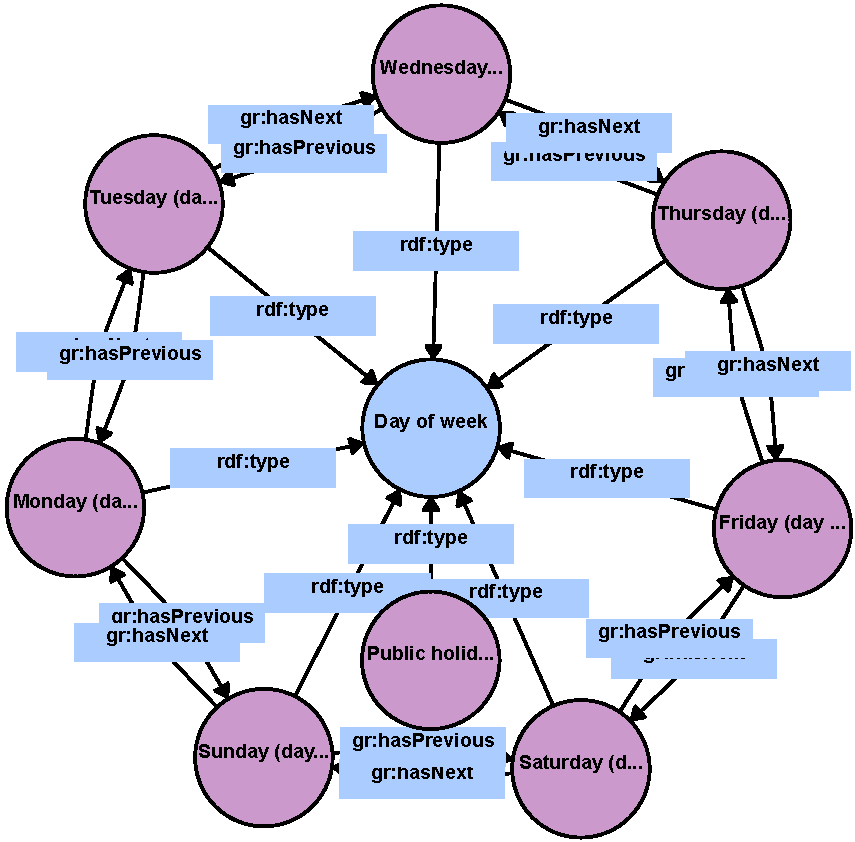
\includegraphics[width=8cm]{figures/code-list-days-of-week}
\caption{Visualization of a simple code list that forms a hierarchy in GoodRelations vocabulary}
\label{fig:code-list-with-hierarchy}
%\vspace{-4mm}
\end{figure}

\subsection{Implementation: Code List Analyzer}

Furthermore, we have implemented a web client called Code List Analyzer, which uses these queries in our workflow to enable a more comprehensive analysis and to provide an empirical insight into the queried data.

The source code of our project is available on GitHub\footnote{\url{https://github.com/nvbach91/iga-hybrid}} under an open-source license. The web client Code List Analyzer is accessible online via \url{https://fcp.vse.cz/iga-hybrid}.

\subsection{Results}

The above sequence of SPARQL queries Q1 through Q5 is implemented in our Code List Analyzer tool and has been successfully executed on a total of 281 LOV vocabularies that have at least one class instance. We have discovered\footnote{\url{https://github.com/nvbach91/iga-hybrid/tree/master/results}} in aggregation that 146 vocabularies do not have any code lists embedded in them. %, probably because these vocabularies are small. 
In 84 vocabularies, there are structures were embedded that resemble code lists. The total number of candidate code lists detected in these vocabularies is 307. 

The top vocabularies that have the highest number of candidate code lists and the top vocabularies that have the highest number of code list members along with their SKOS status are listed in Table \ref{tab:top-codes}.

\begin{table}[h]
\footnotesize
\begin{tabular}{|l|r|l|}
\hline
\textbf{Vocab} & \textbf{Code lists} & \textbf{SKOS} \\ \hline
lexinfo        & 41                  & No \\ \hline
ce*            & 36                  & No \\ \hline
voag           & 22                  & No \\ \hline
bevon          & 18                  & No \\ \hline
topo           & 13                  & Yes \\ \hline
dk             & 12                  & No  \\ \hline
portal         & 9                   & No  \\ \hline
gr             & 9                   & No  \\ \hline
mil            & 9                   & Yes \\ \hline
igeo           & 8                   & Yes \\ \hline
mv*            & 8                   & No  \\ \hline
txn            & 7                   & No  \\ \hline
gvp            & 6                   & No  \\ \hline
opo            & 6                   & No  \\ \hline
itsmo          & 5                   & No  \\ \hline
fresnel        & 5                   & No  \\ \hline
frbr           & 5                   & No  \\ \hline
%ofrd           & 5                   & No  \\ \hline
%vso            & 5                   & No  \\ \hline
%dataid         & 5                   & No  \\ \hline
\end{tabular}
\,
\begin{tabular}{|l|r|l|}
\hline
\textbf{Vocab} & \textbf{Codes} & \textbf{SKOS} \\ \hline
mil             & 732            & Yes    \\ \hline
lexinfo         & 669            & No     \\ \hline
ce*             & 285            & No     \\ \hline
topo            & 233            & Yes    \\ \hline
chord           & 108            & No     \\ \hline
odrl            & 79             & Yes    \\ \hline
voag            & 77             & No     \\ \hline
mv*             & 68             & No     \\ \hline
nlon            & 65             & No     \\ \hline
portal          & 62             & No     \\ \hline
gr              & 47             & No     \\ \hline
txn             & 44             & No     \\ \hline
sport           & 40             & No     \\ \hline
bevon           & 33             & No     \\ \hline
music           & 30             & No     \\ \hline
igeo            & 27             & Yes    \\ \hline
ofrd            & 24             & No     \\ \hline
%dataid          & 23             & No     \\ \hline
%dk              & 18             & No     \\ \hline
%vaem            & 18             & No     \\ \hline
\end{tabular}
\centering
%\captionsetup{justification=centering}
\caption{Top vocabularies with the highest number of embedded code lists and code list members (*ce: consumerelectronics, mv: mobivoc)}
\label{tab:top-codes} 
%\vspace{-6mm}
\end{table}

Another interesting fact is that the numbers of assignment properties are not high for code lists. The highest number of these properties is 3 and there are 4 code lists that have this same number of properties. There are 13 code lists that have 2 assignment properties and 135 code lists that have 1 assignment property. The remaining 155 code lists have 0 assignment properties.

\subsection{Complexity of the process}

The overall query complexity of this SPARQL query sequence can be calculated by multiplying of the number of vocabularies, the number of classes, and the number of instances, since we must repeat the queries that retrieve the instances for each class in each vocabulary. The real-world run-time complexity depends on the database storage implementation. In our case, we directly query against the LOV endpoint, which is powered by the Jena Fuseki triple store \cite{DBLP:journals/semweb/VandenbusscheAP17}, this means that the query speed of Code List Analyzer depends on the query endpoint of LOV. In any case, LOV offers a N-Quads dump, which can be uploaded to any custom triple store of choice and can be run on a local machine.

Considering pattern matching in SPARQL has $\mathcal{O}(\log{}n)$ complexity, the query Q1 should have $\mathcal{O}(n\log{}n)$ complexity to create a list of vocabularies, however, we also calculate here the number of classes and class instances, the complexity becomes $\mathcal{O}(n^3)$. Since query Q2 also retrieves classes and instances, but  depends on the Q1 results (the vocabulary IRI is a parameter of Q2), it will have $\mathcal{O}(n^2)$ complexity. Because of high complexity, these SPARQL queries cannot be combined and must run separately. Therefore, in order to browse the candidate code lists, the users must first select a vocabulary, while having the option to look at the number of class instances, and then select a candidate code list to view the codes.

\subsection{Result visualization}

In our implementation of Code List Analyzer, which can perform these tasks in a semi-automated manner, we have also included WebVOWL \cite{DBLP:journals/semweb/LohmannNHE15} -- a well-known ontology visualization library. The graph visualization helps in obtaining quick insights while viewing the structures of the extracted candidate code lists, especially the relationships between the codes since they are hard to see in tables. We observed that most of the code lists have a flat structure with one class and many individuals on the same instance level as in Figure~\ref{fig:code-list-visualized}.
